% Chapter Template

\chapter{Sprint 0} % Main chapter title

\label{Sprint 0} % Change X to a consecutive number; for referencing this chapter elsewhere, use \ref{ChapterX}

\lhead{Chapter 9. \emph{Sprint 0}} % Change X to a consecutive number; this is for the header on each page - perhaps a shortened title
%This chapter is meant to give an overview of sprint 0. 
%Section 9.1 gies and overview of the planning.
%Section 9.2

\section{Planning}

% ** We planned to have 2 weeks sprint but in the middle of the sprint we changed the first sprint to a 3 week sprint. That makes some of our numebrs inconsistent. Refering to the status reports and the weekly meetings. We usually estimated 60 hours per week of work but the first sprint ended up beeing estimated at 200 hours for 3 weeks**


what we planned to do
shall we include some data from scrumdo? definitely a chart..
\section{Duration}
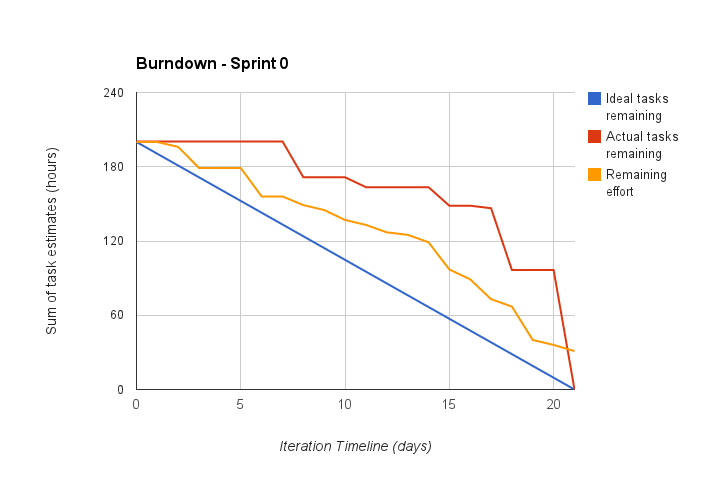
\includegraphics[scale=0.6]{./Figures/burndownSprint0.png}
\section{Goals}
what did we expect to achieve by the end of this sprint (general progress in the project)
\section{Feedback}
from customer, from supervisor
\section{Problems}
\section{Evaluation}
our thoughts about this sprint
